\documentclass[border=8pt]{standalone}
\usepackage{tikz}
\usepackage{amsmath}
\usepackage{amssymb}
\usepackage[scaled=0.92]{helvet}\renewcommand\familydefault{\sfdefault}
\usetikzlibrary{positioning,fit,backgrounds,calc,arrows}

% ---- palette ----
\definecolor{inF}{RGB}{226,233,241}\definecolor{inL}{RGB}{70,90,112}
\definecolor{reF}{RGB}{255,238,208}\definecolor{reL}{RGB}{196,138,38}
\definecolor{eF}{RGB}{214,229,247}\definecolor{eL}{RGB}{38,92,164}
\definecolor{dF}{RGB}{209,238,231}\definecolor{dL}{RGB}{26,132,118}
\definecolor{tF}{RGB}{230,221,243}\definecolor{tL}{RGB}{114,70,162}
\definecolor{cF}{RGB}{219,238,219}\definecolor{cL}{RGB}{56,140,60}
\definecolor{evF}{RGB}{236,236,238}\definecolor{evL}{RGB}{92,92,98}
\definecolor{emF}{RGB}{249,225,225}\definecolor{emL}{RGB}{178,68,68}
\definecolor{arr}{RGB}{70,78,90}

\begin{document}
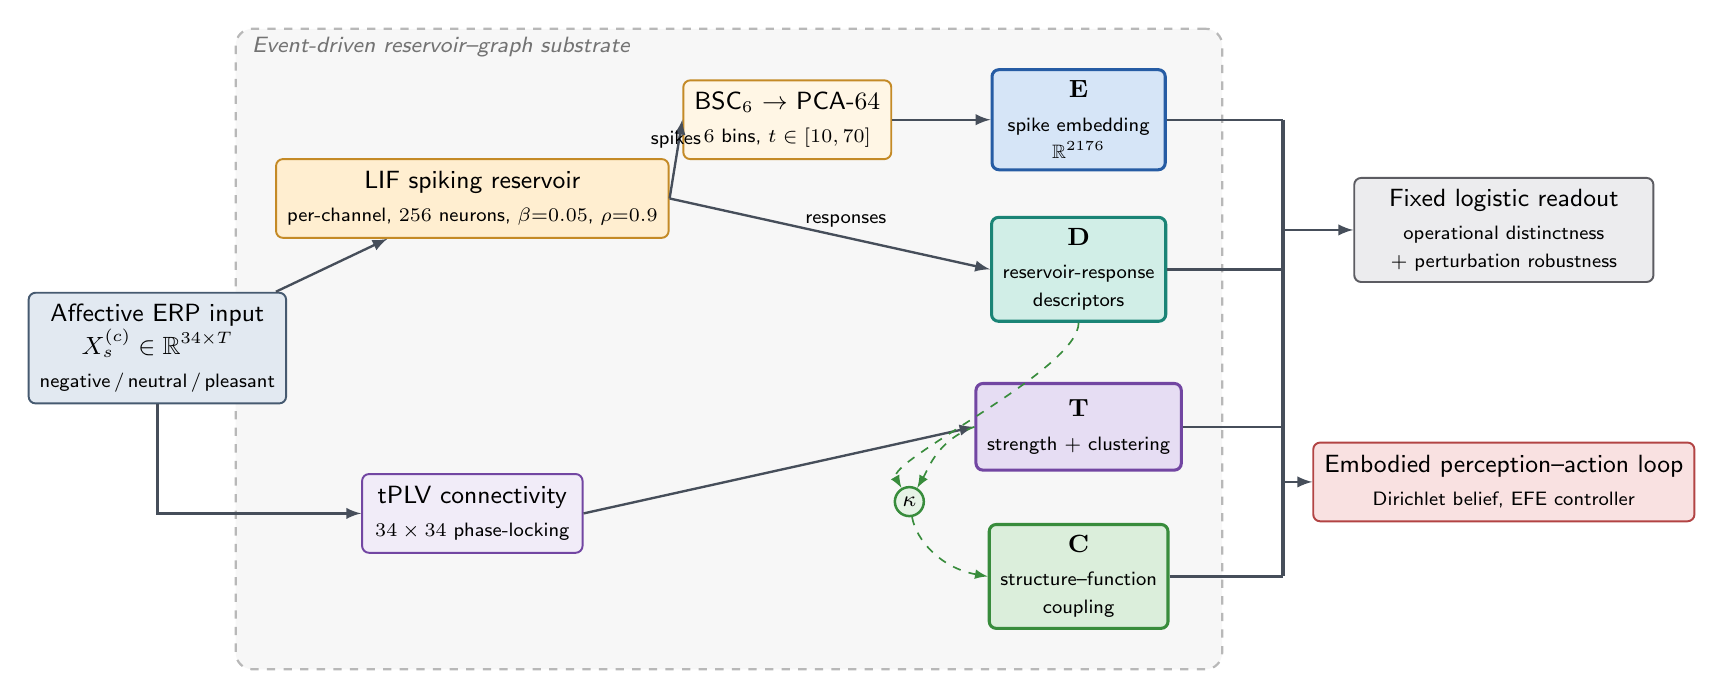
\begin{tikzpicture}[
  font=\small,
  box/.style={rounded corners=2.5pt, draw, line width=0.7pt, align=center, inner sep=4pt, minimum height=10mm},
  io/.style={box, fill=inF, draw=inL, minimum width=24mm},
  re/.style={box, fill=reF, draw=reL, minimum width=30mm},
  proc/.style={box, fill=reF!55, draw=reL, minimum width=26mm},
  conn/.style={box, fill=tF!55, draw=tL, minimum width=28mm},
  chip/.style={rounded corners=2.5pt, draw, line width=1.1pt, align=center, inner sep=4pt, minimum height=11mm, minimum width=22mm},
  ev/.style={box, fill=evF, draw=evL, minimum width=38mm},
  emb/.style={box, fill=emF, draw=emL, minimum width=38mm},
  flow/.style={->, >=latex, line width=0.85pt, draw=arr},
  derive/.style={->, >=latex, line width=0.6pt, draw=cL, dashed},
]

% ---------- nodes ----------
\node[io] (eeg) at (0,0) {Affective ERP input\\[1pt]$X^{(c)}_s\in\mathbb{R}^{34\times T}$\\[1pt]{\scriptsize negative\,/\,neutral\,/\,pleasant}};

\node[re] (res) at (4.0,1.9) {LIF spiking reservoir\\[1pt]{\scriptsize per-channel,\ $256$ neurons,\ $\beta{=}0.05$,\ $\rho{=}0.9$}};
\node[conn] (plv) at (4.0,-2.1) {tPLV connectivity\\[1pt]{\scriptsize $34\times34$ phase-locking}};

\node[proc] (bsc) at (8.0,2.9) {BSC$_6$ $\rightarrow$ PCA-$64$\\[1pt]{\scriptsize $6$ bins,\ $t\in[10,70]$}};

\node[chip, fill=eF, draw=eL] (E) at (11.7,2.9) {$\mathbf{E}$\\[1pt]{\scriptsize spike embedding}\\[-1pt]{\scriptsize $\mathbb{R}^{2176}$}};
\node[chip, fill=dF, draw=dL] (D) at (11.7,1.0) {$\mathbf{D}$\\[1pt]{\scriptsize reservoir-response}\\[-1pt]{\scriptsize descriptors}};
\node[chip, fill=tF, draw=tL] (T) at (11.7,-1.0) {$\mathbf{T}$\\[1pt]{\scriptsize strength $+$ clustering}};
\node[chip, fill=cF, draw=cL] (C) at (11.7,-2.9) {$\mathbf{C}$\\[1pt]{\scriptsize structure--function}\\[-1pt]{\scriptsize coupling}};

\node[circle, draw=cL, fill=cF!70, line width=0.9pt, inner sep=1.6pt, font=\footnotesize] (kap) at (9.55,-1.95) {$\kappa$};

% downstream rail + heads
\node[ev] (read) at (17.1,1.5) {Fixed logistic readout\\[1pt]{\scriptsize operational distinctness}\\[-1pt]{\scriptsize $+$ perturbation robustness}};
\node[emb] (emb) at (17.1,-1.7) {Embodied perception--action loop\\[1pt]{\scriptsize Dirichlet belief,\ EFE controller}};

% ---------- flows ----------
\draw[flow] (eeg) -- (res);
\draw[flow] (eeg.south) |- (plv.west);
\draw[flow] (res.east) -- node[above,font=\scriptsize,pos=0.5]{spikes} (bsc.west);
\draw[flow] (bsc) -- (E);
\draw[flow] (res.east) -- node[above,font=\scriptsize,pos=0.55]{responses} (D.west);
\draw[flow] (plv.east) -- (T.west);

% coupling (derived-from, dashed)
\draw[derive] (D.south) .. controls +(270:6mm) and +(120:6mm) .. (kap);
\draw[derive] (T.west) .. controls +(200:5mm) and +(60:5mm) .. (kap);
\draw[derive] (kap) .. controls +(280:5mm) and +(170:6mm) .. (C.west);

% rail collecting the four streams -> two downstream heads
\coordinate (railx) at (14.3,0);
\draw[line width=0.85pt, draw=arr] (E.east) -- (E.east -| railx);
\draw[line width=0.85pt, draw=arr] (D.east) -- (D.east -| railx);
\draw[line width=0.85pt, draw=arr] (T.east) -- (T.east -| railx);
\draw[line width=0.85pt, draw=arr] (C.east) -- (C.east -| railx);
\draw[line width=1.4pt, draw=arr] (14.3,2.9) -- (14.3,-2.9);
\draw[flow] (read.west -| railx) -- (read.west);
\draw[flow] (emb.west -| railx) -- (emb.west);

% ---------- containers ----------
\begin{scope}[on background layer]
  \node[rounded corners=6pt, fill=black!3, draw=black!28, dashed, line width=0.8pt,
        fit=(res)(plv)(bsc)(E)(D)(T)(C)(kap), inner sep=5mm] (sub) {};
  \node[anchor=north west, font=\footnotesize\itshape, text=black!55] at (sub.north west) {\ Event-driven reservoir--graph substrate};
\end{scope}

\end{tikzpicture}
\end{document}
